\documentclass[border=5pt]{standalone}
\usepackage{fontspec}
\usepackage{unicode-math}
\setmainfont{Noto Serif}
\newfontfamily\FigureItalic{Noto Serif}
\setmathfont{STIXTwoMath-Regular.otf}
\usepackage{tikz}
\usetikzlibrary{arrows.meta,calc,patterns,decorations.pathmorphing,decorations.markings,decorations.pathreplacing,positioning,backgrounds}
\definecolor{Ink}{HTML}{000000}
\definecolor{Curve}{HTML}{000000}
\definecolor{Bzero}{HTML}{000000}
\definecolor{Bone}{HTML}{000000}
\definecolor{Btwo}{HTML}{000000}
\definecolor{Bthree}{HTML}{000000}
\definecolor{Bfour}{HTML}{000000}
\tikzset{
 ax/.style={draw=Ink,line width=.72pt,-{Latex[length=2.4mm,width=1.5mm]}},
 lev/.style={draw=Ink,line width=1.4pt,line cap=butt},
 thinlev/.style={draw=Ink,line width=.65pt,line cap=butt},
 helper/.style={draw=Ink,line width=.65pt},
 bare/.style={draw=Ink,line width=.95pt,dash pattern=on 4pt off 2.8pt},
 curve/.style={draw=Ink,line width=1.85pt,line cap=round,line join=round},
 ray/.style={draw=Ink,line width=1.0pt,-{Latex[length=2.3mm,width=1.4mm]}},
 measure/.style={draw=Ink,line width=.75pt,{Latex[length=1.9mm,width=1.2mm]}-{Latex[length=1.9mm,width=1.2mm]}},
 link/.style={draw=Ink,line width=1.0pt},
 wave/.style={draw=Ink,line width=.85pt,decorate,decoration={snake,amplitude=.33mm,segment length=2.5mm,pre length=.8mm,post length=.8mm}},
 photon/.style={draw=Ink,line width=1.0pt,-{Latex[length=2.0mm,width=1.3mm]},decorate,decoration={snake,amplitude=.4mm,segment length=2.7mm,pre length=0mm,post length=1.9mm}},
 lab/.style={text=Ink,font=\fontsize{13.5}{16}\selectfont,inner sep=2pt},
 small/.style={text=Ink,font=\fontsize{11.5}{14}\selectfont,inner sep=2pt},
 tag/.style={text=Ink,font=\fontsize{14}{17}\selectfont\FigureItalic\itshape,inner sep=2pt}}
\pagestyle{empty}

\begin{document}
% Figure 13.1; source-grounded revision.
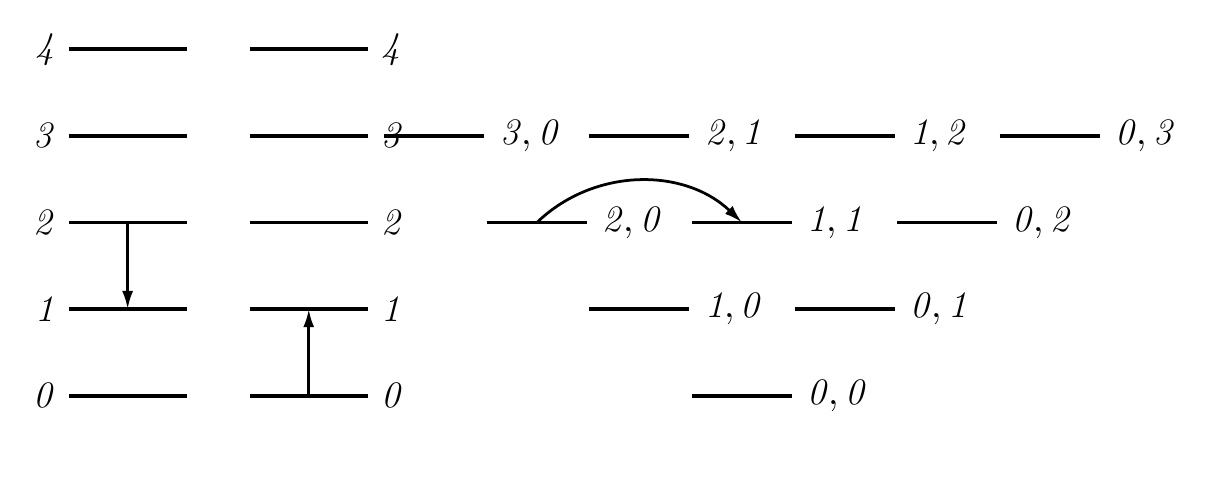
\begin{tikzpicture}[x=1cm,y=1cm]
\coordinate (a00) at (0.90000,0.00000);
\coordinate (a00L) at (0.15000,0.00000);
\coordinate (a00R) at (1.65000,0.00000);
\draw[lev] (a00L) -- (a00R);
\node[lab,anchor=east] at (0.05000,0.00000) {\textit{0}};
\coordinate (a01) at (0.90000,1.10000);
\coordinate (a01L) at (0.15000,1.10000);
\coordinate (a01R) at (1.65000,1.10000);
\draw[lev] (a01L) -- (a01R);
\node[lab,anchor=east] at (0.05000,1.10000) {\textit{1}};
\coordinate (a02) at (0.90000,2.20000);
\coordinate (a02L) at (0.15000,2.20000);
\coordinate (a02R) at (1.65000,2.20000);
\draw[lev] (a02L) -- (a02R);
\node[lab,anchor=east] at (0.05000,2.20000) {\textit{2}};
\coordinate (a03) at (0.90000,3.30000);
\coordinate (a03L) at (0.15000,3.30000);
\coordinate (a03R) at (1.65000,3.30000);
\draw[lev] (a03L) -- (a03R);
\node[lab,anchor=east] at (0.05000,3.30000) {\textit{3}};
\coordinate (a04) at (0.90000,4.40000);
\coordinate (a04L) at (0.15000,4.40000);
\coordinate (a04R) at (1.65000,4.40000);
\draw[lev] (a04L) -- (a04R);
\node[lab,anchor=east] at (0.05000,4.40000) {\textit{4}};
\coordinate (a10) at (3.20000,0.00000);
\coordinate (a10L) at (2.45000,0.00000);
\coordinate (a10R) at (3.95000,0.00000);
\draw[lev] (a10L) -- (a10R);
\node[lab,anchor=west] at (4.05000,0.00000) {\textit{0}};
\coordinate (a11) at (3.20000,1.10000);
\coordinate (a11L) at (2.45000,1.10000);
\coordinate (a11R) at (3.95000,1.10000);
\draw[lev] (a11L) -- (a11R);
\node[lab,anchor=west] at (4.05000,1.10000) {\textit{1}};
\coordinate (a12) at (3.20000,2.20000);
\coordinate (a12L) at (2.45000,2.20000);
\coordinate (a12R) at (3.95000,2.20000);
\draw[lev] (a12L) -- (a12R);
\node[lab,anchor=west] at (4.05000,2.20000) {\textit{2}};
\coordinate (a13) at (3.20000,3.30000);
\coordinate (a13L) at (2.45000,3.30000);
\coordinate (a13R) at (3.95000,3.30000);
\draw[lev] (a13L) -- (a13R);
\node[lab,anchor=west] at (4.05000,3.30000) {\textit{3}};
\coordinate (a14) at (3.20000,4.40000);
\coordinate (a14L) at (2.45000,4.40000);
\coordinate (a14R) at (3.95000,4.40000);
\draw[lev] (a14L) -- (a14R);
\node[lab,anchor=west] at (4.05000,4.40000) {\textit{4}};
\draw[ray] (a02) -- (a01);
\draw[ray] (a10) -- (a11);
\node[tag] at (2.05000,-0.65000) {а};
\begin{scope}[xscale=1.27,xshift=-2.25cm]
\coordinate (s00) at (9.10000,0.00000);
\coordinate (s00L) at (8.60000,0.00000);
\coordinate (s00R) at (9.60000,0.00000);
\draw[lev] (s00L) -- (s00R);
\node[lab,anchor=west] at (9.70000,0.00000) {$\mathit{0,0}$};
\coordinate (s10) at (8.07500,1.10000);
\coordinate (s10L) at (7.57500,1.10000);
\coordinate (s10R) at (8.57500,1.10000);
\draw[lev] (s10L) -- (s10R);
\node[lab,anchor=west] at (8.67500,1.10000) {$\mathit{1,0}$};
\coordinate (s01) at (10.12500,1.10000);
\coordinate (s01L) at (9.62500,1.10000);
\coordinate (s01R) at (10.62500,1.10000);
\draw[lev] (s01L) -- (s01R);
\node[lab,anchor=west] at (10.72500,1.10000) {$\mathit{0,1}$};
\coordinate (s20) at (7.05000,2.20000);
\coordinate (s20L) at (6.55000,2.20000);
\coordinate (s20R) at (7.55000,2.20000);
\draw[lev] (s20L) -- (s20R);
\node[lab,anchor=west] at (7.65000,2.20000) {$\mathit{2,0}$};
\coordinate (s11) at (9.10000,2.20000);
\coordinate (s11L) at (8.60000,2.20000);
\coordinate (s11R) at (9.60000,2.20000);
\draw[lev] (s11L) -- (s11R);
\node[lab,anchor=west] at (9.70000,2.20000) {$\mathit{1,1}$};
\coordinate (s02) at (11.15000,2.20000);
\coordinate (s02L) at (10.65000,2.20000);
\coordinate (s02R) at (11.65000,2.20000);
\draw[lev] (s02L) -- (s02R);
\node[lab,anchor=west] at (11.75000,2.20000) {$\mathit{0,2}$};
\coordinate (s30) at (6.02500,3.30000);
\coordinate (s30L) at (5.52500,3.30000);
\coordinate (s30R) at (6.52500,3.30000);
\draw[lev] (s30L) -- (s30R);
\node[lab,anchor=west] at (6.62500,3.30000) {$\mathit{3,0}$};
\coordinate (s21) at (8.07500,3.30000);
\coordinate (s21L) at (7.57500,3.30000);
\coordinate (s21R) at (8.57500,3.30000);
\draw[lev] (s21L) -- (s21R);
\node[lab,anchor=west] at (8.67500,3.30000) {$\mathit{2,1}$};
\coordinate (s12) at (10.12500,3.30000);
\coordinate (s12L) at (9.62500,3.30000);
\coordinate (s12R) at (10.62500,3.30000);
\draw[lev] (s12L) -- (s12R);
\node[lab,anchor=west] at (10.72500,3.30000) {$\mathit{1,2}$};
\coordinate (s03) at (12.17500,3.30000);
\coordinate (s03L) at (11.67500,3.30000);
\coordinate (s03R) at (12.67500,3.30000);
\draw[lev] (s03L) -- (s03R);
\node[lab,anchor=west] at (12.77500,3.30000) {$\mathit{0,3}$};
\draw[ray] (s20) .. controls (7.62400,2.90000) and (8.52600,2.90000) .. (s11);
\node[tag] at (9.10000,-0.65000) {б};
\end{scope}\end{tikzpicture}

\end{document}
